\begin{figure}
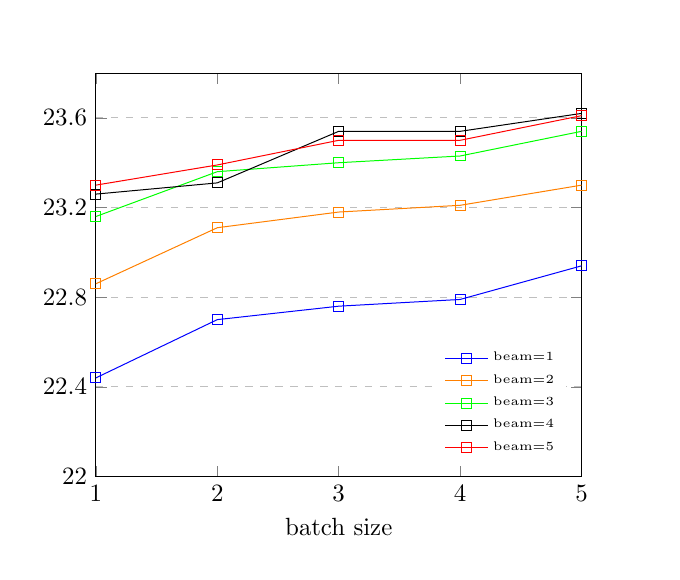
\begin{tikzpicture}
\scalebox{0.9}{
\begin{axis}[
    %title={BLEU},
    xlabel={batch size},
    %ylabel={},
    xmin=1, xmax=5,
    ymin=22, ymax=23.8,
    xtick={1,2,3,4,5},
    ytick={22.0,22.4,22.8,23.2,23.6},
    legend pos=south east,
    %legend style={font=\fontsize{4}{5}\selectfont},
    legend style={font=\tiny, draw=none},
    ymajorgrids=true,
    grid style=dashed,
]
 
\addplot[
    color=blue,
    mark=square,
    ]
    coordinates {
    (1,22.44)	(2,22.7)	(3,22.76)	(4,22.79)	(5,22.94)
    };

\addplot[
    color=orange,
    mark=square,
    ]
    coordinates {
    (1,22.86)	(2,23.11)	(3,23.18)	(4,23.21)	(5,23.3)
    };
    
\addplot[
    color=green,
    mark=square,
    ]
    coordinates {
    (1,23.16)	(2,23.36)	(3,23.4)	(4,23.43)	(5,23.54)
    };

\addplot[
    color=black,
    mark=square,
    ]
    coordinates {
    (1,23.26)	(2,23.31)	(3,23.54)	(4,23.54)	(5,23.62)
    };

\addplot[
    color=red,
    mark=square,
    ]
    coordinates {
    (1,23.3)	(2,23.39)	(3,23.5)	(4,23.5)	(5,23.61)
    };

    \legend{beam=1, beam=2, beam=3, beam=4, beam=5}
 
\end{axis}
}
\end{tikzpicture}
\caption{BLEU evaluations on different beam size and batch size}
\label{fig:beam_batch_bleu}
\end{figure}
